\documentclass[1p]{elsarticle_modified}
%\bibliographystyle{elsarticle-num}

%\usepackage[colorlinks]{hyperref}
%\usepackage{abbrmath_seonhwa} %\Abb, \Ascr, \Acal ,\Abf, \Afrak
\usepackage{amsfonts}
\usepackage{amssymb}
\usepackage{amsmath}
\usepackage{amsthm}
\usepackage{scalefnt}
\usepackage{amsbsy}
\usepackage{kotex}
\usepackage{caption}
\usepackage{subfig}
\usepackage{color}
\usepackage{graphicx}
\usepackage{xcolor} %% white, black, red, green, blue, cyan, magenta, yellow
\usepackage{float}
\usepackage{setspace}
\usepackage{hyperref}

\usepackage{tikz}
\usetikzlibrary{arrows}

\usepackage{multirow}
\usepackage{array} % fixed length table
\usepackage{hhline}

%%%%%%%%%%%%%%%%%%%%%
\makeatletter
\renewcommand*\env@matrix[1][\arraystretch]{%
	\edef\arraystretch{#1}%
	\hskip -\arraycolsep
	\let\@ifnextchar\new@ifnextchar
	\array{*\c@MaxMatrixCols c}}
\makeatother %https://tex.stackexchange.com/questions/14071/how-can-i-increase-the-line-spacing-in-a-matrix
%%%%%%%%%%%%%%%

\usepackage[normalem]{ulem}

\newcommand{\msout}[1]{\ifmmode\text{\sout{\ensuremath{#1}}}\else\sout{#1}\fi}
%SOURCE: \msout is \stkout macro in https://tex.stackexchange.com/questions/20609/strikeout-in-math-mode

\newcommand{\cancel}[1]{
	\ifmmode
	{\color{red}\msout{#1}}
	\else
	{\color{red}\sout{#1}}
	\fi
}

\newcommand{\add}[1]{
	{\color{blue}\uwave{#1}}
}

\newcommand{\replace}[2]{
	\ifmmode
	{\color{red}\msout{#1}}{\color{blue}\uwave{#2}}
	\else
	{\color{red}\sout{#1}}{\color{blue}\uwave{#2}}
	\fi
}

\newcommand{\Sol}{\mathcal{S}} %segment
\newcommand{\D}{D} %diagram
\newcommand{\A}{\mathcal{A}} %arc


%%%%%%%%%%%%%%%%%%%%%%%%%%%%%5 test

\def\sl{\operatorname{\textup{SL}}(2,\Cbb)}
\def\psl{\operatorname{\textup{PSL}}(2,\Cbb)}
\def\quan{\mkern 1mu \triangleright \mkern 1mu}

\theoremstyle{definition}
\newtheorem{thm}{Theorem}[section]
\newtheorem{prop}[thm]{Proposition}
\newtheorem{lem}[thm]{Lemma}
\newtheorem{ques}[thm]{Question}
\newtheorem{cor}[thm]{Corollary}
\newtheorem{defn}[thm]{Definition}
\newtheorem{exam}[thm]{Example}
\newtheorem{rmk}[thm]{Remark}
\newtheorem{alg}[thm]{Algorithm}

\newcommand{\I}{\sqrt{-1}}
\begin{document}

%\begin{frontmatter}
%
%\title{Boundary parabolic representations of knots up to 8 crossings}
%
%%% Group authors per affiliation:
%\author{Yunhi Cho} 
%\address{Department of Mathematics, University of Seoul, Seoul, Korea}
%\ead{yhcho@uos.ac.kr}
%
%
%\author{Seonhwa Kim} %\fnref{s_kim}}
%\address{Center for Geometry and Physics, Institute for Basic Science, Pohang, 37673, Korea}
%\ead{ryeona17@ibs.re.kr}
%
%\author{Hyuk Kim}
%\address{Department of Mathematical Sciences, Seoul National University, Seoul 08826, Korea}
%\ead{hyukkim@snu.ac.kr}
%
%\author{Seokbeom Yoon}
%\address{Department of Mathematical Sciences, Seoul National University, Seoul, 08826,  Korea}
%\ead{sbyoon15@snu.ac.kr}
%
%\begin{abstract}
%We find all boundary parabolic representation of knots up to 8 crossings.
%
%\end{abstract}
%\begin{keyword}
%    \MSC[2010] 57M25 
%\end{keyword}
%
%\end{frontmatter}

%\linenumbers
%\tableofcontents
%
\newcommand\colored[1]{\textcolor{white}{\rule[-0.35ex]{0.8em}{1.4ex}}\kern-0.8em\color{red} #1}%
%\newcommand\colored[1]{\textcolor{white}{ #1}\kern-2.17ex	\textcolor{white}{ #1}\kern-1.81ex	\textcolor{white}{ #1}\kern-2.15ex\color{red}#1	}

{\Large $\underline{12n_{0077}~(K12n_{0077})}$}

\setlength{\tabcolsep}{10pt}
\renewcommand{\arraystretch}{1.6}
\vspace{1cm}\begin{tabular}{m{100pt}>{\centering\arraybackslash}m{274pt}}
\multirow{5}{120pt}{
	\centering
	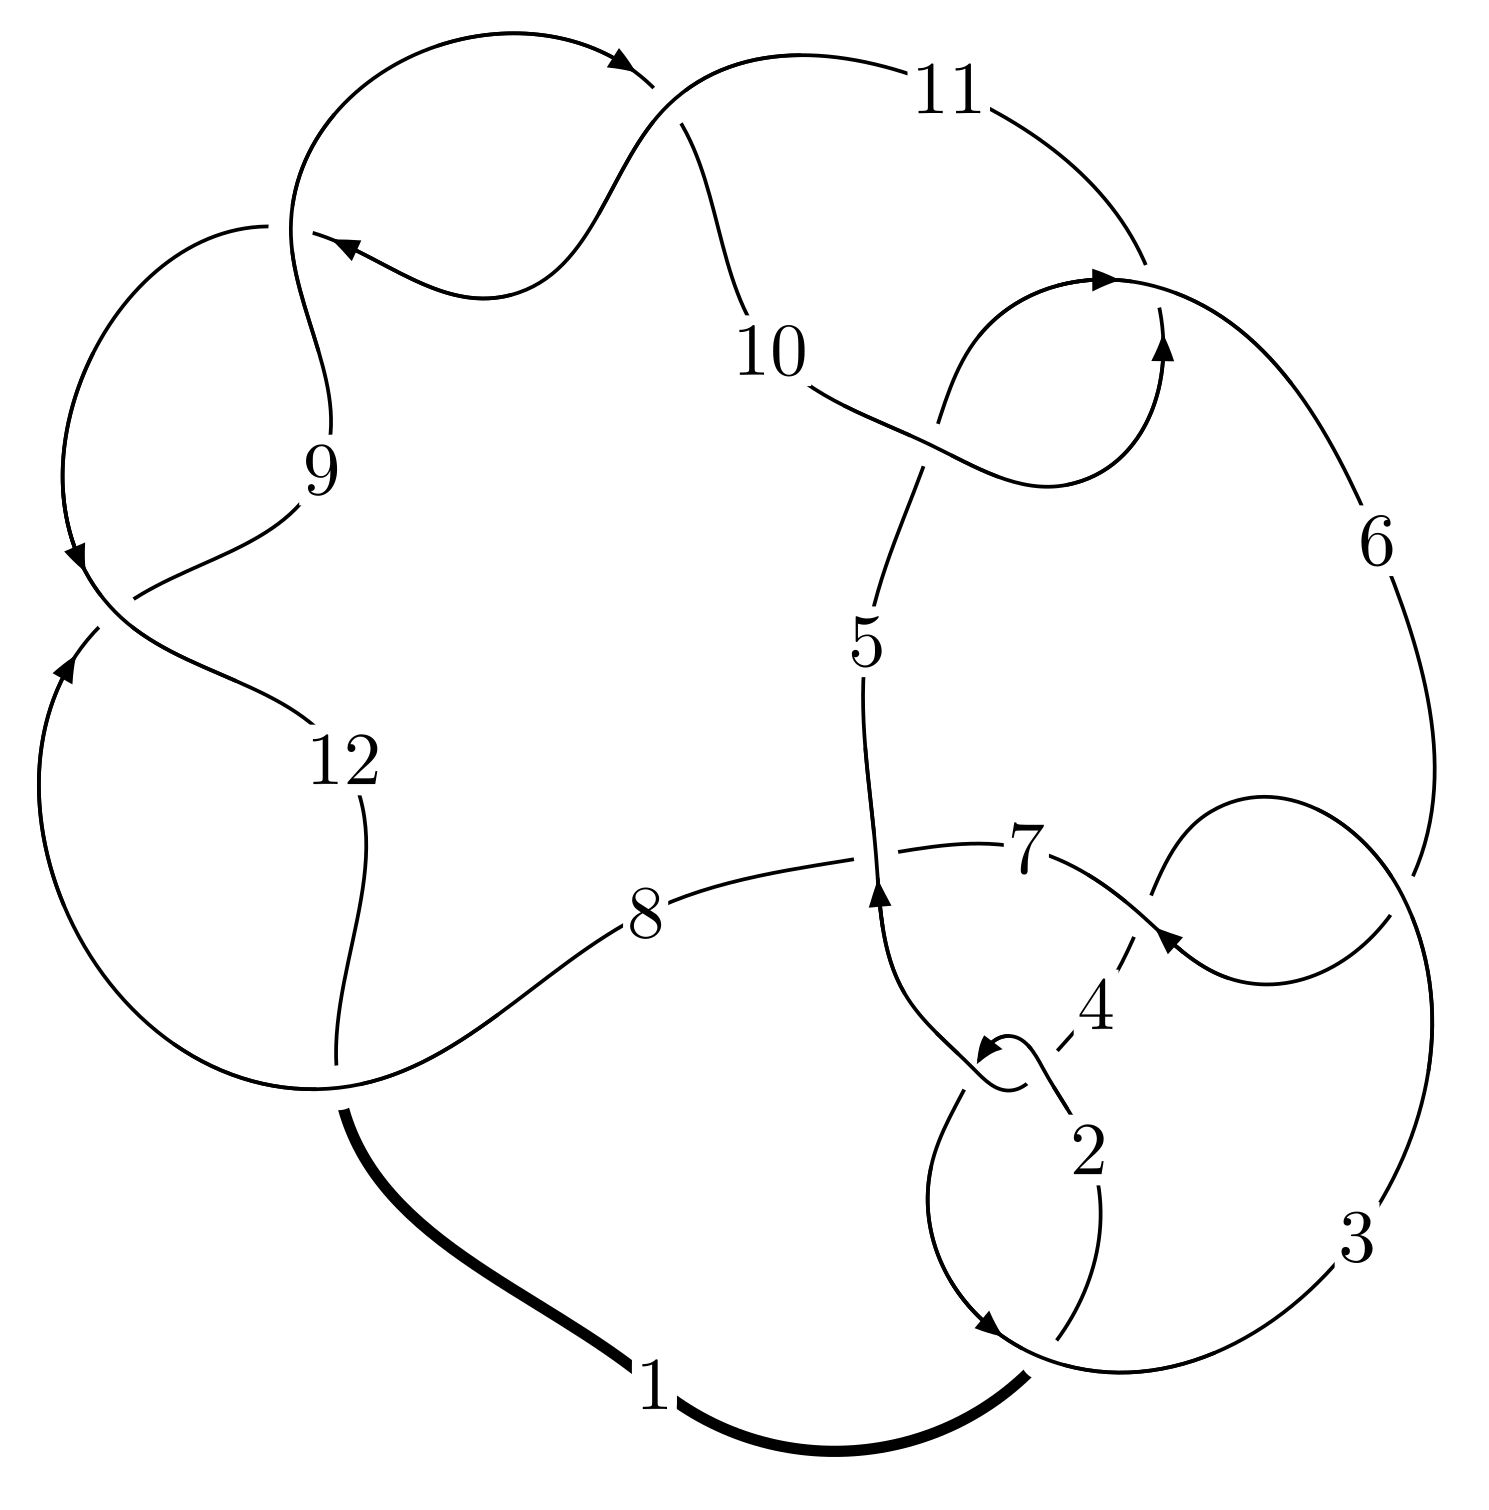
\includegraphics[width=112pt]{../../../GIT/diagram.site/Diagrams/png/2166_12n_0077.png}\\
\ \ \ A knot diagram\footnotemark}&
\allowdisplaybreaks
\textbf{Linearized knot diagam} \\
\cline{2-2}
 &
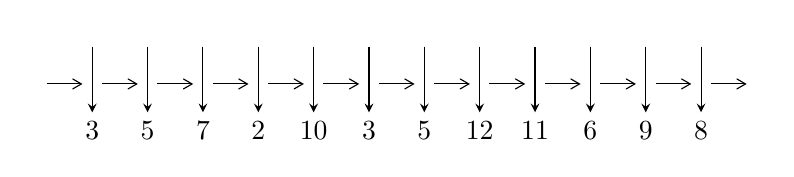
\begin{tikzpicture}[x=20pt, y=17pt]
	% nodes
	\node (C0) at (0, 0) {};
	\node (C1) at (1, 0) {};
	\node (C1U) at (1, +1) {};
	\node (C1D) at (1, -1) {3};

	\node (C2) at (2, 0) {};
	\node (C2U) at (2, +1) {};
	\node (C2D) at (2, -1) {5};

	\node (C3) at (3, 0) {};
	\node (C3U) at (3, +1) {};
	\node (C3D) at (3, -1) {7};

	\node (C4) at (4, 0) {};
	\node (C4U) at (4, +1) {};
	\node (C4D) at (4, -1) {2};

	\node (C5) at (5, 0) {};
	\node (C5U) at (5, +1) {};
	\node (C5D) at (5, -1) {10};

	\node (C6) at (6, 0) {};
	\node (C6U) at (6, +1) {};
	\node (C6D) at (6, -1) {3};

	\node (C7) at (7, 0) {};
	\node (C7U) at (7, +1) {};
	\node (C7D) at (7, -1) {5};

	\node (C8) at (8, 0) {};
	\node (C8U) at (8, +1) {};
	\node (C8D) at (8, -1) {12};

	\node (C9) at (9, 0) {};
	\node (C9U) at (9, +1) {};
	\node (C9D) at (9, -1) {11};

	\node (C10) at (10, 0) {};
	\node (C10U) at (10, +1) {};
	\node (C10D) at (10, -1) {6};

	\node (C11) at (11, 0) {};
	\node (C11U) at (11, +1) {};
	\node (C11D) at (11, -1) {9};

	\node (C12) at (12, 0) {};
	\node (C12U) at (12, +1) {};
	\node (C12D) at (12, -1) {8};
	\node (C13) at (13, 0) {};

	% arrows
	\draw[->,>={angle 60}]
	(C0) edge (C1) (C1) edge (C2) (C2) edge (C3) (C3) edge (C4) (C4) edge (C5) (C5) edge (C6) (C6) edge (C7) (C7) edge (C8) (C8) edge (C9) (C9) edge (C10) (C10) edge (C11) (C11) edge (C12) (C12) edge (C13) ;	\draw[->,>=stealth]
	(C1U) edge (C1D) (C2U) edge (C2D) (C3U) edge (C3D) (C4U) edge (C4D) (C5U) edge (C5D) (C6U) edge (C6D) (C7U) edge (C7D) (C8U) edge (C8D) (C9U) edge (C9D) (C10U) edge (C10D) (C11U) edge (C11D) (C12U) edge (C12D) ;
	\end{tikzpicture} \\
\hhline{~~} \\& 
\textbf{Solving Sequence} \\ \cline{2-2} 
 &
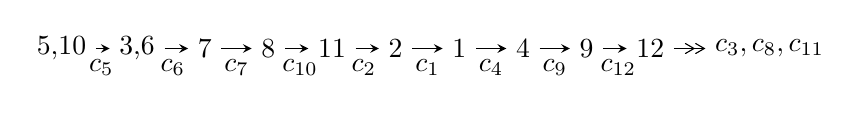
\begin{tikzpicture}[x=23pt, y=7pt]
	% node
	\node (A0) at (-1/8, 0) {5,10};
	\node (A1) at (17/16, 0) {3,6};
	\node (A2) at (17/8, 0) {7};
	\node (A3) at (25/8, 0) {8};
	\node (A4) at (33/8, 0) {11};
	\node (A5) at (41/8, 0) {2};
	\node (A6) at (49/8, 0) {1};
	\node (A7) at (57/8, 0) {4};
	\node (A8) at (65/8, 0) {9};
	\node (A9) at (73/8, 0) {12};
	\node (C1) at (1/2, -1) {$c_{5}$};
	\node (C2) at (13/8, -1) {$c_{6}$};
	\node (C3) at (21/8, -1) {$c_{7}$};
	\node (C4) at (29/8, -1) {$c_{10}$};
	\node (C5) at (37/8, -1) {$c_{2}$};
	\node (C6) at (45/8, -1) {$c_{1}$};
	\node (C7) at (53/8, -1) {$c_{4}$};
	\node (C8) at (61/8, -1) {$c_{9}$};
	\node (C9) at (69/8, -1) {$c_{12}$};
	\node (A10) at (11, 0) {$c_{3},c_{8},c_{11}$};

	% edge
	\draw[->,>=stealth]	
	(A0) edge (A1) (A1) edge (A2) (A2) edge (A3) (A3) edge (A4) (A4) edge (A5) (A5) edge (A6) (A6) edge (A7) (A7) edge (A8) (A8) edge (A9) ;
	\draw[->>,>={angle 60}]	
	(A9) edge (A10);
\end{tikzpicture} \\ 

\end{tabular} \\

\footnotetext{
The image of knot diagram is generated by the software ``\textbf{Draw programme}" developed by Andrew Bartholomew(\url{http://www.layer8.co.uk/maths/draw/index.htm\#Running-draw}), where we modified some parts for our purpose(\url{https://github.com/CATsTAILs/LinksPainter}).
}\phantom \\ \newline 
\centering \textbf{Ideals for irreducible components\footnotemark of $X_{\text{par}}$} 
 
\begin{align*}
I^u_{1}&=\langle 
u^{25}- u^{24}+\cdots+b+1,\;u^{22}-3 u^{20}+\cdots+a+4 u,\;u^{26}-2 u^{25}+\cdots-2 u-1\rangle \\
I^u_{2}&=\langle 
b+1,\;u^4- u^2+a+u+2,\;u^5- u^4+u^2+u-1\rangle \\
\\
\end{align*}
\raggedright * 2 irreducible components of $\dim_{\mathbb{C}}=0$, with total 31 representations.\\
\footnotetext{All coefficients of polynomials are rational numbers. But the coefficients are sometimes approximated in decimal forms when there is not enough margin.}
\newpage
\renewcommand{\arraystretch}{1}
\centering \section*{I. $I^u_{1}= \langle u^{25}- u^{24}+\cdots+b+1,\;u^{22}-3 u^{20}+\cdots+a+4 u,\;u^{26}-2 u^{25}+\cdots-2 u-1 \rangle$}
\flushleft \textbf{(i) Arc colorings}\\
\begin{tabular}{m{7pt} m{180pt} m{7pt} m{180pt} }
\flushright $a_{5}=$&$\begin{pmatrix}1\\0\end{pmatrix}$ \\
\flushright $a_{10}=$&$\begin{pmatrix}0\\u\end{pmatrix}$ \\
\flushright $a_{3}=$&$\begin{pmatrix}- u^{22}+3 u^{20}+\cdots-4 u^2-4 u\\- u^{25}+u^{24}+\cdots- u-1\end{pmatrix}$ \\
\flushright $a_{6}=$&$\begin{pmatrix}1\\u^2\end{pmatrix}$ \\
\flushright $a_{7}=$&$\begin{pmatrix}- u^9-3 u^5- u\\- u^9+u^7-3 u^5+2 u^3- u\end{pmatrix}$ \\
\flushright $a_{8}=$&$\begin{pmatrix}- u^7-2 u^3\\- u^9+u^7-3 u^5+2 u^3- u\end{pmatrix}$ \\
\flushright $a_{11}=$&$\begin{pmatrix}- u\\- u^3+u\end{pmatrix}$ \\
\flushright $a_{2}=$&$\begin{pmatrix}- u^{25}+u^{24}+\cdots-5 u-1\\- u^{25}+u^{24}+\cdots- u-1\end{pmatrix}$ \\
\flushright $a_{1}=$&$\begin{pmatrix}- u^9-3 u^5- u\\- u^{11}+u^9-4 u^7+3 u^5-3 u^3+u\end{pmatrix}$ \\
\flushright $a_{4}=$&$\begin{pmatrix}-2 u^{25}+2 u^{24}+\cdots-7 u-1\\- u^{25}+u^{24}+\cdots-2 u-1\end{pmatrix}$ \\
\flushright $a_{9}=$&$\begin{pmatrix}u^3\\u^5- u^3+u\end{pmatrix}$ \\
\flushright $a_{12}=$&$\begin{pmatrix}- u^5- u\\- u^7+u^5-2 u^3+u\end{pmatrix}$\\&\end{tabular}
\flushleft \textbf{(ii) Obstruction class $= -1$}\\~\\
\flushleft \textbf{(iii) Cusp Shapes $= -2 u^{25}+u^{24}+8 u^{23}-10 u^{22}-26 u^{21}+30 u^{20}+57 u^{19}-86 u^{18}-103 u^{17}+156 u^{16}+148 u^{15}-242 u^{14}-181 u^{13}+278 u^{12}+205 u^{11}-248 u^{10}-197 u^9+159 u^8+194 u^7-60 u^6-148 u^5+8 u^4+77 u^3+10 u^2-19 u-20$}\\~\\
\newpage\renewcommand{\arraystretch}{1}
\flushleft \textbf{(iv) u-Polynomials at the component}\newline \\
\begin{tabular}{m{50pt}|m{274pt}}
Crossings & \hspace{64pt}u-Polynomials at each crossing \\
\hline $$\begin{aligned}c_{1}\end{aligned}$$&$\begin{aligned}
&u^{26}+34 u^{25}+\cdots+68 u+1
\end{aligned}$\\
\hline $$\begin{aligned}c_{2},c_{4}\end{aligned}$$&$\begin{aligned}
&u^{26}-6 u^{25}+\cdots+34 u^2-1
\end{aligned}$\\
\hline $$\begin{aligned}c_{3},c_{6}\end{aligned}$$&$\begin{aligned}
&u^{26}+u^{25}+\cdots+96 u+32
\end{aligned}$\\
\hline $$\begin{aligned}c_{5},c_{10}\end{aligned}$$&$\begin{aligned}
&u^{26}-2 u^{25}+\cdots-2 u-1
\end{aligned}$\\
\hline $$\begin{aligned}c_{7}\end{aligned}$$&$\begin{aligned}
&u^{26}-2 u^{25}+\cdots-2 u-1
\end{aligned}$\\
\hline $$\begin{aligned}c_{8},c_{9},c_{11}\\c_{12}\end{aligned}$$&$\begin{aligned}
&u^{26}+6 u^{25}+\cdots+10 u+1
\end{aligned}$\\
\hline
\end{tabular}\\~\\
\newpage\renewcommand{\arraystretch}{1}
\flushleft \textbf{(v) Riley Polynomials at the component}\newline \\
\begin{tabular}{m{50pt}|m{274pt}}
Crossings & \hspace{64pt}Riley Polynomials at each crossing \\
\hline $$\begin{aligned}c_{1}\end{aligned}$$&$\begin{aligned}
&y^{26}-78 y^{25}+\cdots-1224 y+1
\end{aligned}$\\
\hline $$\begin{aligned}c_{2},c_{4}\end{aligned}$$&$\begin{aligned}
&y^{26}-34 y^{25}+\cdots-68 y+1
\end{aligned}$\\
\hline $$\begin{aligned}c_{3},c_{6}\end{aligned}$$&$\begin{aligned}
&y^{26}-33 y^{25}+\cdots-1536 y+1024
\end{aligned}$\\
\hline $$\begin{aligned}c_{5},c_{10}\end{aligned}$$&$\begin{aligned}
&y^{26}-6 y^{25}+\cdots-10 y+1
\end{aligned}$\\
\hline $$\begin{aligned}c_{7}\end{aligned}$$&$\begin{aligned}
&y^{26}-54 y^{25}+\cdots-10 y+1
\end{aligned}$\\
\hline $$\begin{aligned}c_{8},c_{9},c_{11}\\c_{12}\end{aligned}$$&$\begin{aligned}
&y^{26}+30 y^{25}+\cdots+18 y+1
\end{aligned}$\\
\hline
\end{tabular}\\~\\
\newpage\flushleft \textbf{(vi) Complex Volumes and Cusp Shapes}
$$\begin{array}{c|c|c}  
\text{Solutions to }I^u_{1}& \I (\text{vol} + \sqrt{-1}CS) & \text{Cusp shape}\\
 \hline 
\begin{aligned}
u &= \phantom{-}1.03768\phantom{ +0.000000I} \\
a &= \phantom{-}3.52363\phantom{ +0.000000I} \\
b &= \phantom{-}1.79564\phantom{ +0.000000I}\end{aligned}
 & -14.3257\phantom{ +0.000000I} & -18.8510\phantom{ +0.000000I} \\ \hline\begin{aligned}
u &= -0.848363 + 0.365549 I \\
a &= -1.78442 - 1.39985 I \\
b &= -0.876527 + 0.552462 I\end{aligned}
 & -2.09559 + 3.16364 I & -16.0021 - 6.5670 I \\ \hline\begin{aligned}
u &= -0.848363 - 0.365549 I \\
a &= -1.78442 + 1.39985 I \\
b &= -0.876527 - 0.552462 I\end{aligned}
 & -2.09559 - 3.16364 I & -16.0021 + 6.5670 I \\ \hline\begin{aligned}
u &= \phantom{-}0.743105 + 0.536823 I \\
a &= \phantom{-}0.594036 - 0.232636 I \\
b &= \phantom{-}0.265907 - 0.097994 I\end{aligned}
 & \phantom{-}1.42344 - 2.05884 I & -4.65256 + 4.58362 I \\ \hline\begin{aligned}
u &= \phantom{-}0.743105 - 0.536823 I \\
a &= \phantom{-}0.594036 + 0.232636 I \\
b &= \phantom{-}0.265907 + 0.097994 I\end{aligned}
 & \phantom{-}1.42344 + 2.05884 I & -4.65256 - 4.58362 I \\ \hline\begin{aligned}
u &= -1.016900 + 0.465737 I \\
a &= \phantom{-}2.21366 + 1.97366 I \\
b &= \phantom{-}1.76028 - 0.15334 I\end{aligned}
 & -11.56550 + 6.15142 I & -15.5995 - 5.2395 I \\ \hline\begin{aligned}
u &= -1.016900 - 0.465737 I \\
a &= \phantom{-}2.21366 - 1.97366 I \\
b &= \phantom{-}1.76028 + 0.15334 I\end{aligned}
 & -11.56550 - 6.15142 I & -15.5995 + 5.2395 I \\ \hline\begin{aligned}
u &= -0.340992 + 0.772246 I \\
a &= \phantom{-}0.190362 - 0.001300 I \\
b &= \phantom{-}1.70063 + 0.08748 I\end{aligned}
 & -9.33177 - 1.67049 I & -11.65109 + 0.28027 I \\ \hline\begin{aligned}
u &= -0.340992 - 0.772246 I \\
a &= \phantom{-}0.190362 + 0.001300 I \\
b &= \phantom{-}1.70063 - 0.08748 I\end{aligned}
 & -9.33177 + 1.67049 I & -11.65109 - 0.28027 I \\ \hline\begin{aligned}
u &= \phantom{-}0.780793 + 0.228604 I \\
a &= -2.51035 + 0.76802 I \\
b &= -1.168300 + 0.232886 I\end{aligned}
 & -2.90735 - 0.78726 I & -17.0746 + 5.9643 I\\
 \hline 
 \end{array}$$\newpage$$\begin{array}{c|c|c}  
\text{Solutions to }I^u_{1}& \I (\text{vol} + \sqrt{-1}CS) & \text{Cusp shape}\\
 \hline 
\begin{aligned}
u &= \phantom{-}0.780793 - 0.228604 I \\
a &= -2.51035 - 0.76802 I \\
b &= -1.168300 - 0.232886 I\end{aligned}
 & -2.90735 + 0.78726 I & -17.0746 - 5.9643 I \\ \hline\begin{aligned}
u &= -0.901624 + 0.824241 I \\
a &= -0.978749 - 0.966956 I \\
b &= -1.49560 - 0.03445 I\end{aligned}
 & \phantom{-}3.16228 + 3.07757 I & -10.53156 - 2.75315 I \\ \hline\begin{aligned}
u &= -0.901624 - 0.824241 I \\
a &= -0.978749 + 0.966956 I \\
b &= -1.49560 + 0.03445 I\end{aligned}
 & \phantom{-}3.16228 - 3.07757 I & -10.53156 + 2.75315 I \\ \hline\begin{aligned}
u &= \phantom{-}0.875285 + 0.858337 I \\
a &= \phantom{-}0.452866 - 0.465694 I \\
b &= -0.617869 + 0.854688 I\end{aligned}
 & \phantom{-}5.39540 - 0.25204 I & -9.68980 - 0.25577 I \\ \hline\begin{aligned}
u &= \phantom{-}0.875285 - 0.858337 I \\
a &= \phantom{-}0.452866 + 0.465694 I \\
b &= -0.617869 - 0.854688 I\end{aligned}
 & \phantom{-}5.39540 + 0.25204 I & -9.68980 + 0.25577 I \\ \hline\begin{aligned}
u &= \phantom{-}0.840955 + 0.925824 I \\
a &= \phantom{-}0.193479 + 0.004136 I \\
b &= \phantom{-}1.65874 - 0.26853 I\end{aligned}
 & -2.27912 + 3.95861 I & -11.45131 - 0.83940 I \\ \hline\begin{aligned}
u &= \phantom{-}0.840955 - 0.925824 I \\
a &= \phantom{-}0.193479 - 0.004136 I \\
b &= \phantom{-}1.65874 + 0.26853 I\end{aligned}
 & -2.27912 - 3.95861 I & -11.45131 + 0.83940 I \\ \hline\begin{aligned}
u &= \phantom{-}0.939409 + 0.834109 I \\
a &= -0.76938 + 1.23390 I \\
b &= -0.687301 - 0.869387 I\end{aligned}
 & \phantom{-}5.19384 - 6.03805 I & -10.26289 + 5.25215 I \\ \hline\begin{aligned}
u &= \phantom{-}0.939409 - 0.834109 I \\
a &= -0.76938 - 1.23390 I \\
b &= -0.687301 + 0.869387 I\end{aligned}
 & \phantom{-}5.19384 + 6.03805 I & -10.26289 - 5.25215 I \\ \hline\begin{aligned}
u &= -0.931297 + 0.895111 I \\
a &= \phantom{-}0.372833 + 0.308620 I \\
b &= \phantom{-}0.537292 + 0.017409 I\end{aligned}
 & \phantom{-}10.10520 + 3.30342 I & -2.39471 - 2.26919 I\\
 \hline 
 \end{array}$$\newpage$$\begin{array}{c|c|c}  
\text{Solutions to }I^u_{1}& \I (\text{vol} + \sqrt{-1}CS) & \text{Cusp shape}\\
 \hline 
\begin{aligned}
u &= -0.931297 - 0.895111 I \\
a &= \phantom{-}0.372833 - 0.308620 I \\
b &= \phantom{-}0.537292 - 0.017409 I\end{aligned}
 & \phantom{-}10.10520 - 3.30342 I & -2.39471 + 2.26919 I \\ \hline\begin{aligned}
u &= \phantom{-}0.998011 + 0.849444 I \\
a &= \phantom{-}0.83951 - 1.88704 I \\
b &= \phantom{-}1.68410 + 0.28961 I\end{aligned}
 & -2.78496 - 10.50130 I & -12.09690 + 5.41863 I \\ \hline\begin{aligned}
u &= \phantom{-}0.998011 - 0.849444 I \\
a &= \phantom{-}0.83951 + 1.88704 I \\
b &= \phantom{-}1.68410 - 0.28961 I\end{aligned}
 & -2.78496 + 10.50130 I & -12.09690 - 5.41863 I \\ \hline\begin{aligned}
u &= -0.527536\phantom{ +0.000000I} \\
a &= \phantom{-}0.849795\phantom{ +0.000000I} \\
b &= -0.171524\phantom{ +0.000000I}\end{aligned}
 & -0.708379\phantom{ +0.000000I} & -14.2100\phantom{ +0.000000I} \\ \hline\begin{aligned}
u &= -0.393456 + 0.342390 I \\
a &= \phantom{-}0.999444 + 0.387392 I \\
b &= -0.573413 - 0.271251 I\end{aligned}
 & -0.780751 - 0.150062 I & -11.06268 - 0.12594 I \\ \hline\begin{aligned}
u &= -0.393456 - 0.342390 I \\
a &= \phantom{-}0.999444 - 0.387392 I \\
b &= -0.573413 + 0.271251 I\end{aligned}
 & -0.780751 + 0.150062 I & -11.06268 + 0.12594 I\\
 \hline 
 \end{array}$$\newpage\newpage\renewcommand{\arraystretch}{1}
\centering \section*{II. $I^u_{2}= \langle b+1,\;u^4- u^2+a+u+2,\;u^5- u^4+u^2+u-1 \rangle$}
\flushleft \textbf{(i) Arc colorings}\\
\begin{tabular}{m{7pt} m{180pt} m{7pt} m{180pt} }
\flushright $a_{5}=$&$\begin{pmatrix}1\\0\end{pmatrix}$ \\
\flushright $a_{10}=$&$\begin{pmatrix}0\\u\end{pmatrix}$ \\
\flushright $a_{3}=$&$\begin{pmatrix}- u^4+u^2- u-2\\-1\end{pmatrix}$ \\
\flushright $a_{6}=$&$\begin{pmatrix}1\\u^2\end{pmatrix}$ \\
\flushright $a_{7}=$&$\begin{pmatrix}1\\u^2\end{pmatrix}$ \\
\flushright $a_{8}=$&$\begin{pmatrix}- u^2+1\\u^2\end{pmatrix}$ \\
\flushright $a_{11}=$&$\begin{pmatrix}- u\\- u^3+u\end{pmatrix}$ \\
\flushright $a_{2}=$&$\begin{pmatrix}- u^4+u^2- u-3\\-1\end{pmatrix}$ \\
\flushright $a_{1}=$&$\begin{pmatrix}-1\\0\end{pmatrix}$ \\
\flushright $a_{4}=$&$\begin{pmatrix}- u^4+u^2- u-2\\-1\end{pmatrix}$ \\
\flushright $a_{9}=$&$\begin{pmatrix}u^3\\u^4- u^3- u^2+1\end{pmatrix}$ \\
\flushright $a_{12}=$&$\begin{pmatrix}- u^4+u^2-1\\u^4\end{pmatrix}$\\&\end{tabular}
\flushleft \textbf{(ii) Obstruction class $= 1$}\\~\\
\flushleft \textbf{(iii) Cusp Shapes $= - u^3+3 u^2- u-14$}\\~\\
\newpage\renewcommand{\arraystretch}{1}
\flushleft \textbf{(iv) u-Polynomials at the component}\newline \\
\begin{tabular}{m{50pt}|m{274pt}}
Crossings & \hspace{64pt}u-Polynomials at each crossing \\
\hline $$\begin{aligned}c_{1},c_{2}\end{aligned}$$&$\begin{aligned}
&(u-1)^5
\end{aligned}$\\
\hline $$\begin{aligned}c_{3},c_{6}\end{aligned}$$&$\begin{aligned}
&u^5
\end{aligned}$\\
\hline $$\begin{aligned}c_{4}\end{aligned}$$&$\begin{aligned}
&(u+1)^5
\end{aligned}$\\
\hline $$\begin{aligned}c_{5}\end{aligned}$$&$\begin{aligned}
&u^5- u^4+u^2+u-1
\end{aligned}$\\
\hline $$\begin{aligned}c_{7},c_{11},c_{12}\end{aligned}$$&$\begin{aligned}
&u^5+u^4+4 u^3+3 u^2+3 u+1
\end{aligned}$\\
\hline $$\begin{aligned}c_{8},c_{9}\end{aligned}$$&$\begin{aligned}
&u^5- u^4+4 u^3-3 u^2+3 u-1
\end{aligned}$\\
\hline $$\begin{aligned}c_{10}\end{aligned}$$&$\begin{aligned}
&u^5+u^4- u^2+u+1
\end{aligned}$\\
\hline
\end{tabular}\\~\\
\newpage\renewcommand{\arraystretch}{1}
\flushleft \textbf{(v) Riley Polynomials at the component}\newline \\
\begin{tabular}{m{50pt}|m{274pt}}
Crossings & \hspace{64pt}Riley Polynomials at each crossing \\
\hline $$\begin{aligned}c_{1},c_{2},c_{4}\end{aligned}$$&$\begin{aligned}
&(y-1)^5
\end{aligned}$\\
\hline $$\begin{aligned}c_{3},c_{6}\end{aligned}$$&$\begin{aligned}
&y^5
\end{aligned}$\\
\hline $$\begin{aligned}c_{5},c_{10}\end{aligned}$$&$\begin{aligned}
&y^5- y^4+4 y^3-3 y^2+3 y-1
\end{aligned}$\\
\hline $$\begin{aligned}c_{7},c_{8},c_{9}\\c_{11},c_{12}\end{aligned}$$&$\begin{aligned}
&y^5+7 y^4+16 y^3+13 y^2+3 y-1
\end{aligned}$\\
\hline
\end{tabular}\\~\\
\newpage\flushleft \textbf{(vi) Complex Volumes and Cusp Shapes}
$$\begin{array}{c|c|c}  
\text{Solutions to }I^u_{2}& \I (\text{vol} + \sqrt{-1}CS) & \text{Cusp shape}\\
 \hline 
\begin{aligned}
u &= -0.758138 + 0.584034 I \\
a &= -0.278580 - 1.055720 I \\
b &= -1.00000\phantom{ +0.000000I}\end{aligned}
 & \phantom{-}0.17487 + 2.21397 I & -12.88087 - 4.04855 I \\ \hline\begin{aligned}
u &= -0.758138 - 0.584034 I \\
a &= -0.278580 + 1.055720 I \\
b &= -1.00000\phantom{ +0.000000I}\end{aligned}
 & \phantom{-}0.17487 - 2.21397 I & -12.88087 + 4.04855 I \\ \hline\begin{aligned}
u &= \phantom{-}0.935538 + 0.903908 I \\
a &= -0.020316 + 0.590570 I \\
b &= -1.00000\phantom{ +0.000000I}\end{aligned}
 & \phantom{-}9.31336 - 3.33174 I & -13.28666 + 2.53508 I \\ \hline\begin{aligned}
u &= \phantom{-}0.935538 - 0.903908 I \\
a &= -0.020316 - 0.590570 I \\
b &= -1.00000\phantom{ +0.000000I}\end{aligned}
 & \phantom{-}9.31336 + 3.33174 I & -13.28666 - 2.53508 I \\ \hline\begin{aligned}
u &= \phantom{-}0.645200\phantom{ +0.000000I} \\
a &= -2.40221\phantom{ +0.000000I} \\
b &= -1.00000\phantom{ +0.000000I}\end{aligned}
 & -2.52712\phantom{ +0.000000I} & -13.6650\phantom{ +0.000000I}\\
 \hline 
 \end{array}$$\newpage
\newpage\renewcommand{\arraystretch}{1}
\centering \section*{ III. u-Polynomials}
\begin{tabular}{m{50pt}|m{274pt}}
Crossings & \hspace{64pt}u-Polynomials at each crossing \\
\hline $$\begin{aligned}c_{1}\end{aligned}$$&$\begin{aligned}
&((u-1)^5)(u^{26}+34 u^{25}+\cdots+68 u+1)
\end{aligned}$\\
\hline $$\begin{aligned}c_{2}\end{aligned}$$&$\begin{aligned}
&((u-1)^5)(u^{26}-6 u^{25}+\cdots+34 u^2-1)
\end{aligned}$\\
\hline $$\begin{aligned}c_{3},c_{6}\end{aligned}$$&$\begin{aligned}
&u^5(u^{26}+u^{25}+\cdots+96 u+32)
\end{aligned}$\\
\hline $$\begin{aligned}c_{4}\end{aligned}$$&$\begin{aligned}
&((u+1)^5)(u^{26}-6 u^{25}+\cdots+34 u^2-1)
\end{aligned}$\\
\hline $$\begin{aligned}c_{5}\end{aligned}$$&$\begin{aligned}
&(u^5- u^4+u^2+u-1)(u^{26}-2 u^{25}+\cdots-2 u-1)
\end{aligned}$\\
\hline $$\begin{aligned}c_{7}\end{aligned}$$&$\begin{aligned}
&(u^5+u^4+4 u^3+3 u^2+3 u+1)(u^{26}-2 u^{25}+\cdots-2 u-1)
\end{aligned}$\\
\hline $$\begin{aligned}c_{8},c_{9}\end{aligned}$$&$\begin{aligned}
&(u^5- u^4+4 u^3-3 u^2+3 u-1)(u^{26}+6 u^{25}+\cdots+10 u+1)
\end{aligned}$\\
\hline $$\begin{aligned}c_{10}\end{aligned}$$&$\begin{aligned}
&(u^5+u^4- u^2+u+1)(u^{26}-2 u^{25}+\cdots-2 u-1)
\end{aligned}$\\
\hline $$\begin{aligned}c_{11},c_{12}\end{aligned}$$&$\begin{aligned}
&(u^5+u^4+4 u^3+3 u^2+3 u+1)(u^{26}+6 u^{25}+\cdots+10 u+1)
\end{aligned}$\\
\hline
\end{tabular}\newpage\renewcommand{\arraystretch}{1}
\centering \section*{ IV. Riley Polynomials}
\begin{tabular}{m{50pt}|m{274pt}}
Crossings & \hspace{64pt}Riley Polynomials at each crossing \\
\hline $$\begin{aligned}c_{1}\end{aligned}$$&$\begin{aligned}
&((y-1)^5)(y^{26}-78 y^{25}+\cdots-1224 y+1)
\end{aligned}$\\
\hline $$\begin{aligned}c_{2},c_{4}\end{aligned}$$&$\begin{aligned}
&((y-1)^5)(y^{26}-34 y^{25}+\cdots-68 y+1)
\end{aligned}$\\
\hline $$\begin{aligned}c_{3},c_{6}\end{aligned}$$&$\begin{aligned}
&y^5(y^{26}-33 y^{25}+\cdots-1536 y+1024)
\end{aligned}$\\
\hline $$\begin{aligned}c_{5},c_{10}\end{aligned}$$&$\begin{aligned}
&(y^5- y^4+4 y^3-3 y^2+3 y-1)(y^{26}-6 y^{25}+\cdots-10 y+1)
\end{aligned}$\\
\hline $$\begin{aligned}c_{7}\end{aligned}$$&$\begin{aligned}
&(y^5+7 y^4+16 y^3+13 y^2+3 y-1)(y^{26}-54 y^{25}+\cdots-10 y+1)
\end{aligned}$\\
\hline $$\begin{aligned}c_{8},c_{9},c_{11}\\c_{12}\end{aligned}$$&$\begin{aligned}
&(y^5+7 y^4+16 y^3+13 y^2+3 y-1)(y^{26}+30 y^{25}+\cdots+18 y+1)
\end{aligned}$\\
\hline
\end{tabular}
\vskip 2pc
\end{document}